\documentclass[a4paper,10pt]{article}


\usepackage[utf8]{inputenc}
%\usepackage{mathtools}
\usepackage{graphicx}
\usepackage[italian]{babel}
%\usepackage{float}
%\usepackage{amsmath}
\usepackage{verbatim}

\title{Analisi ponte trifase total-controllato}
\author{Olivieri Daniele}
\date{18 novembre 2019}

\pdfinfo{%
  /Title    (Analisi ponte trifase total-controllato)
  /Author   (Olivieri Daniele)
  /Creator  ()
  /Producer ()
  /Subject  (Elettronica di Potenza)
  /Keywords (FEP, Power Electronics, Three Phase Converter)
}

\begin{document}
\maketitle

\begin{abstract}
 ciao ciao
\end{abstract}

\begin{comment}
\section{Introduzione} %C'è l'abstract come introduzione(?)
Elenco canali oscilloscopio:
1 - Giallo: Vl sul carico
2 - Verde: Vr sulla resistenza o corrente nel carico
3 - Blu: corrente al secondario
4 - Rosso: corrente al primario

Trasformatore stella con neutro al primario - stella al secondario
\end{comment}


\section{Norme tecniche che disciplinano la procedura di prova}
Il comitato tecnico che disciplina l'elettronica di potenza è il CT 22 e la norma
di riferimento per la prova è la CEI EN 60146 ``Convertitori a semiconduttore''.

\section{Strumenti utilizzati}
Per effettuare la prova sono stati utilizzati i seguenti strumenti di misura:
\begin{itemize}
 \item Oscilloscopio a 4 canali Keysight DSO-X 2014A
 \item Trasduttore di corrente ad effetto Hall da 5 A, artigianale
\end{itemize}

\section{Componenti utilizzati}

\section{Schema elettrico del circuito di prova}
\begin{figure}[h]
 \centering
 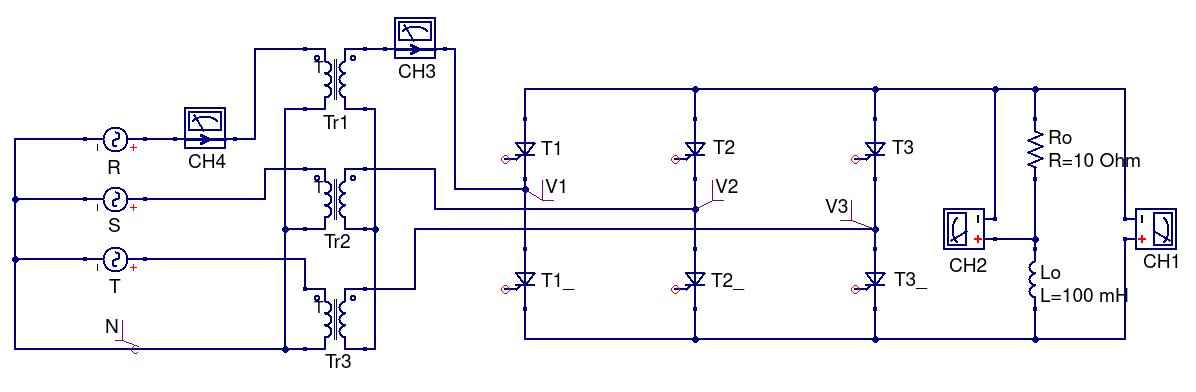
\includegraphics[keepaspectratio=true,width=1\linewidth]{img/circuito_qucs.png}
 % circuito_qucs.png: 1193x395 px, 115dpi, 26.35x8.72 cm, bb=0 0 747 247
 \label{Fig.:}
\end{figure}

\section{Richiami teorici}

\section{Descrizione della prova eseguita}

\section{Risultati ottenuti}

\end{document}
